\documentclass{article}
\usepackage[final]{neurips_2018}
\usepackage[utf8]{inputenc} % allow utf-8 input
\usepackage[T1]{fontenc}    % use 8-bit T1 fonts
\usepackage{hyperref}       % hyperlinks
\usepackage{url}            % simple URL typesetting
\usepackage{booktabs}       % professional-quality tables
\usepackage{amsfonts}       % blackboard math symbols
\usepackage{nicefrac}       % compact symbols for 1/2, etc.
\usepackage{microtype}      % microtypography

\title{Deep Rendering}
\author{Mark Wesley Harris\\
University of Colorado\\
Colorado Springs\\
\texttt{wharris2@uccs.edu} \\
\And
Semwal Sudhanshu\\
University of Colorado\\
Colorado Springs\\
\texttt{ssemwal@uccs.edu} \\
}

\begin{document}

\maketitle

\begin{abstract}
We propose a new render pipeline that combines current research in deep learning
to generate realistic, high-resolution renderings of 3D scenes.
\end{abstract}

\section{Hypothesis}
\label{sec:hypothesis}

\subsection{Research Questions}
\label{subsec:questions}
\begin{enumerate}
\item Is it possible to create a system to generate frames dynamically, based off of previous rendered data and previously un-rendered frames?
\item How much resolution or quality can be expected using such an approach?
\item Does the relevance of previously rendered frames impact how the pipeline handles new inputs?
\item How efficient could the proposed system be, compared to the outputs of current rendering technologies?
\item Where else might this pipeline be applied?
\end{enumerate}

\subsection{Proposed Methodology}
\label{subsec:methodology}
\begin{enumerate}
\item Research current technologies
\item Draft a pipeline that could work in theory
\item Apply current knowledge and previous researched architectures to the drafted pipeline
\item Create sample input data, including rendered frames (or pieces of frames) with corresponding binary from the source scene
\end{enumerate}

\section{Introduction}
\label{sec:introduction}
Even state-of-the-art machines struggle with rendering a 3-dimensional scene. This is due to the preprocessing and computations which must occur for each artifact in the scene and every pixel of the screen. The problem is exacerbated further for higher resolution renderings, wherein millions of objects are present in the scene being rendered.

Researchers are now turning to deep learning and other advanced techniques in order to produce images. The Generative Adversarial Network (GAN) was first
proposed by \cite{gan}.
The GAN was first proposed as a way to train a model to produce
more realistic images. The network is made up of two architectures:
a generator, $G$, and a discriminator, $D$.
GANs are able to generate new images that have similar qualities to
those in the dataset which they are trained on
\cite{generative_adversarial_networks}.

\begin{figure}[htbp]
\centerline{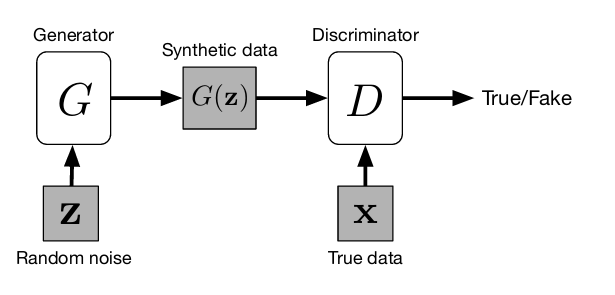
\includegraphics[width=7cm]{gan_architecture.png}}
\caption{Basic Generative Adversarial Network architecture, with a generator $G$
and discriminator $D$
\cite{cgan}.}
\label{fig:gan_architecture}
\end{figure}

The generalized GAN architecture is shown in Figure \ref{fig:gan_architecture}.
The model works by training both the generator $G$ and
discriminator $D$ in tandem.
$G$ is trained to progressively generate more realistic images,
while $D$ is trained to recognize differences between real and fake inputs.
This relationship can be expressed in the format of a
``two-player min-max game'', shown in Equation \ref{eq:gan_basic}.
Here, $p_{data}(\mathbf{x})$ represents the true data distribution,
and $p_{z}(\mathbf{z})$ represents the distribution of noise.
The goal in training a GAN is to minimize error in the generator
and maximize error detection in the discriminator \cite{cgan}.
Optimizations and variants can be made from this simple concept, of which include
the implementations of cGAN, DCGAN, and SRGAN.

\begin{equation}
\label{eq:gan_basic}
\begin{split}
\text{min}_G\text{max}_DV(D,G) &=
E_{\mathbf{x}\sim p_{data}(\mathbf{x})}[\log D(\mathbf{x})] \\
&+ E_{\mathbf{z}\sim p_{z}(\mathbf{z})}[\log(1 - D(G(\mathbf{z})))]
\end{split}
\end{equation}

\section{Related Work}
\label{sec:related}

\subsection*{Pose Guided Person Image Generation, 2017}
\nocite{pg2}
This paper discusses the development of the Pose Guided Person Generation
Network (PG\textsuperscript{2}). PG\textsuperscript{2} contains two stages:
the first is a generative network using several stacked convolutional layers,
which generates an initial course output;
the second is a similar generative network that refines the
result of the previous stage. By combining both of these,
the authors show that it is possible to produce withstanding results of
high similarity to the subject positioned in the target pose.
Ma et al. use a U-Net architecture for the generators, and a discriminator
similar to that used in the DCGAN created by
\cite{unsupervised_representational}.

The PG\textsuperscript{2} architecture is very relevant to our proposed work,
however there are a few key differences. The ``target pose'' that was used as 
part of the inputs of the first generator is represented in a visual format,
specifically a black and white image with a series of nodes representing the
pose. This standardized representation was also used to mask the reference image,
thereby disregarding data irrelevant to the network.
The generator was thus trained to learn the relationship between two
images -- a target pose and masked input pose. We assert that the complexity of a
scene, which must take into account all objects both
inside and outside the camera's view, cannot be represented in the same format.
%This is evident from the sophistication of current rendering pipelines, which
%make use of ray tracing and Monte Carlo sampling to produce their output.
It is possible that multiple images representing a panoramic view of the scene
could be used, however obtaining these would eliminate the advantages of deep
rendering altogether. To compensate, we propose using semantic scene data in the
form of text. The work of Ma et al. is still be very useful in determining the
foundation for our proposed network and its components.
%It is unclear whether this text-to-image process will be as fruitful as the
%image-to-image technique employed by Ma et al.

\subsection*{Multi-View Image Generation from a Single-View, 2018}
\nocite{multi_view}
The architecture covered in this paper is similar to that of PG
\textsuperscript{2}
discussed previously; it is also comprised of two generative
networks, and was evaluated in its ability to create a new view of a given pose.
Zhao et al. argue that it is difficult for basic Generative Adversarial Networks
(GANs) to learn global structures, which is why they implemented what they
call VariGANs. VariGANs use
``\dots variation inference for modeling correct contours and adversarial
learning to fill realistic details'' \cite{multi_view}. The complete architecture
is similar to PG\textsuperscript{2}, but uses primitive word embedding instead of
a standardized representation for inputting conditional data into the coarse
generator. They also only use one conditional discriminator instead of a 
discriminator per generative network.

Although the results of their evaluation were not as good as those with
PG\textsuperscript{2}, Zhao et al. include valuable insights for
our proposed work. If nothing else, we will study the differences between the two
generative models. The claimed success of both works provides reassurance for our
proposed network architecture, which relies on conditional data in the form of
text instead of in image format.

\subsection*{Learn, Imagine and Create: Text-to-Image Generation from Prior Knowledge, 2019}
\nocite{leica}
Qiao et al. combine Attention with concepts from GANs to create what they call
LEarn, Imagine and CreAte GAN (LeicaGAN). Similar to the papers discussed
previously, their architecture is comprised of a coarse image generator followed
by a fine image generator. The main difference for the LeicaGAN is their use
of textual-visual co-embedding (TVE) and multiple priors aggregation (MPA)
to further extract semantic meaning from their inputs. Qiao et al. argue that
their network more closely models how the human brain analyzes textual data,
and therefore will have better results in identifying the relationships between
an image and its textual description.

The LeicaGAN was not evaluated in the same way as the PG\textsuperscript{2} and
the VariGAN architectures; instead of converting one image to another, they
generate a novel image off of textual input alone. In this sense, the LeicaGAN
is the most relevant research to our proposed work. However, since the results
are more arbitrary, it is possible the network could fail in recognizing the
precise representations and complexities within a scene as a whole.
We propose first using the coarse image generator of the LeicaGAN architecture,
and later applying the work from other architectures to try to improve
our results.

\subsection*{Image-to-Image Translation with Conditional Adversarial Networks, 2017}
\nocite{pix2pix}
Isola et al. show that a conditional GAN (cGAN) architecture can be used to
convert from one type of image to another; examples include edges to photograph,
day to night, and black and white to color. The constructed architecture, called
Pix2Pix, uses a U-Net like structure similar to what Ma et al. developed for
PG\textsuperscript{2}. However, the Pix2Pix discriminator network is modeled off
of the Makovian discriminator created by \cite{markovian},
referred to herein as PatchGAN.
The goal of PatchGAN is to disregard meaning from lower frequency structures,
thereby capturing global phenomenon. Isola et al. argue that this discriminator
schema trains the generator to create crisper output images with finer details.

Pix2Pix was evaluated using 9 different tasks. While not all of their
experiments showed improvements from existing technologies, it is noteworthy
in itself that a single network could learn 9 or more types of image conversion.
One of their experiments included converting semantic labels to photographs,
which is particularly relevant to our proposed work.
Pix2Pix falls into the category of image-to-image conversion, which implies that
their achievements may not be directly applicable to our proposed research.
Despite this, we expect that the notable improvements on their discriminator 
architecture could also be applied to our proposed network improve the results
of the generative models.

\subsection*{Blockwise Multi-Order Feature Regression for Real-Time Path Tracing Reconstruction, 2019}
\nocite{path_tracing}
Path tracing is such a computationally intensive process that contemporary
frameworks
``\dots are able to produce only around one path tracing sample per pixel (spp)
at real-time frame rates'' \cite{path_tracing}.
To alleviate this problem, Koskela et al. propose using a
Blockwise Multi-Order Feature Regression (BMFR) algorithm.
As explained, BMFR creates a non-linear fit with respect to the
features of a 1 spp path-traced
frame. They also include a preprocessing stage where frame data (including
spacial positions and normals) from previous frames is accumulated to improve
temporal stability of noise. The results of their experiments showed
improvements upon current real-time methods for certain aspects of the image
(such as soft shadows) and also in regards to calculated loss measurements.

Much like the previously discussed research, external data was incorporated
in an image format. The results obtained by Koskela et al. may serve as a basis
for the argument that image data could in fact be used if it is expressive enough
for training.
While the BMFR algorithm is not an end-to-end solution for us, we may still find
worth in how they up-sampled a low-resolution input frame. In this regard,
we must consider our options for image refinement beyond deep learning.
For now we plan to use a Super Resolution GAN architecture; however, depending on
our final results, BMFR or an alternative algorithm could be
applied to further refine or correct anomalies.

\subsection*{3D Point Capsule Networks, 2019}
\nocite{point_capsule}
As discussed previously, one of the most prevalent problems in processing raw 3D
scene data is accurately capturing the relationships inherent to the data itself.
Zhao et al. designed a network architecture to encapsulate this information into
learned objects of data. Their architecture, called 3D-PointCapsNet,
builds upon the recent research of 2D capsule networks (CNs).
They state that their 3D-PointCapsNet architecture functions as
``\dots an auto-encoder for generic representation
learning in unstructured 3D data'' \cite{point_capsule}. The network was trained
to recognize spatial arrangements of 3D point cloud data, as well as perform
numerous tasks such as part segmentation and configuration interpolation.

This work is promising for the future of 3D shape processing, however its
implications on rendering are yet to be uncovered. Nonetheless, Zhao et al.
proved through their experiments that point capsules could be used to
aid a network in learning the complexities inherent to 3D data, and as such
could be beneficial to our proposed work. A full application of point capsules
as done in 3D-PointCapsNet would disregard the segmented nature of the scene and
likely also the connections between the scene and rendered frame.
We plan to apply their work in discussion on how textual data can be encapsulated
for better learning for our generative networks.

\subsection*{Geometry-Based Next Frame Prediction from Monocular Video, 2017}
\nocite{frame_prediction}
A topic very close to our proposed work is that of frame prediction --
instead of filling in missing frames, the goal of prediction is to create a novel
output based on all previous input data.
Mahjourian, Wicke, and Angelova create a Long Short-Term Memory (LSTM) network
which consumes previous frame information and outputs a depth prediction of the
frame. They then generate the next frame off of the depth prediction, in the same
way as the methods improved upon by Isola et al., in applying Pix2Pix to convert 
one type of image into another.

The existing results of the LSTM network are close to the
target output, but include gaps where the densities are unknown.
We believe the approach can be generalized to support the premise of
the work by Koskela et al. and Isola et al.;
it is possible to convert a meaningful semantic representation
of image data into novel image, while withholding the semantic relationship
between source data and rendered frame. Mahjourian, Wicke, and Angelova show that
LSTM architectures would prove useful for temporally related data,
including the source frames we plan to use in our proposed work.

\section{Methodology}
\label{sec:methodology}

\subsection{Approach}
\label{subsec:approach}

\subsection{Timeline}
\label{subsec:timeline}

\bibliography{proposal}
\bibliographystyle{aaai}

\end{document}
